\subsection{How to Implement Features?}
\begin{frame}{\myframetitle}
	\begin{mycolumns}
		\myexampletight{Given a Feature Model for Graphs \ldots}{
			\centering\featureDiagramGraphs
			%\featureDiagramLegend
		}
		\myexample{\ldots and a Valid Configuration}{
			\small
			\leftmiddleandright{
				$\{G\}$\\
				$\{G,C\}$\\
				$\{G,D\}$\\
				$\{G,C,D\}$\\
			}{
				$\{G,W\}$\\
				$\{G,C,W\}$\\
				$\{G,D,W\}$\\
				$\{G,C,D,W\}$\\
			}{
				$\{G,W,S\}$\\
				$\{G,C,W,S\}$\\
				$\{G,D,W,S\}$\\
				$\{G,C,D,W,S\}$\\
			}
		}
	\mynextcolumn
		\vspace{-10mm}
		\myexampletight{How to Generate Products Automatically?}{
			\centering\foreach \page in {2,12,4,14,6,16,8,18,10,20,42,44}{\includegraphics[width=.23\linewidth,page=\page]{graphs} }
		}
		\mynote{Goals}{
			\begin{itemize}
				\item descriptive specification of a product (i.e., a configuration, a selection of features)
				\item automated generation of a product with compile-time variability
			\end{itemize}
			Focus of the next three lectures \ldots
		}
	\end{mycolumns}
\end{frame}

\subsection{Problems of Ad-Hoc Approaches for Variability}
\subsubsection{Features with Runtime Variability?}
% feature model used to create valid configuration
% configuration used to generate global variables/configuration files/runtime parameters
% automated generation, but no compile-time variability

\subsubsection{Features with Clone-and-Own?}
% compile-time variability, but ...
% no automated generation with version control
% automated generation with build systems but no features

\subsection{Introducing Features to Build Systems}

\subsection{KBuild -- The Linux Kernel Build System}
% https://docs.kernel.org/kbuild/kbuild.html

\subsection{Discussion of Features with Build Systems}

%\begin{frame}{\myframetitle}
%	\begin{mycolumns}
%		\todots
%	\mynextcolumn
%		\todots
%	\end{mycolumns}
%\end{frame}
